\documentclass{beamer-control}
\usepackage{beamer-control-singlefile}
\INCLUDEONLY{Stability Margins}
\begin{document}
\CONCEPT{Stability Margins}

\begin{SUMMARY}
\begin{itemize}
\item Descriptions of stability
\item Calculating stability margins
\end{itemize}
\vfill References:
\begin{itemize}
\item \astrom{§10.3}
\end{itemize}
\end{SUMMARY}



\SUBCONCEPT{Descriptions of stability}

\begin{frame}{How stable is a system?}
\begin{itemize}
\item The Nyquist criterion tells us when a system will be unstable in closed loop -- dependent on encirclement of the critical point
\item In practice, a system may be stable but very close to instability and so we would like a way to capture how far from instability a system is
\item Stability margins express how well the Nyquist curve of a system avoids the critical point by representing how much gain or phase must be added to the system to make it unstable
\item This tells us how robust the system is to perturbation or control parameters
\end{itemize}
\end{frame}



\begin{frame}{Different margins}
There are three types of margin to assess stability
\begin{itemize}
	\item The stability margin $s_m$ describes the shortest distance of the Nyquist curve to the critical point
	\item As increasing the controller gain expands the Nyquist curve radially, the gain margin $g_m$ is defined as the smallest multiplier of the loop gain that makes the system unstable (recommended range $2<g_m<5$)
	\item As increasing the phase of the controller turns the Nyquist curve clockwise, the phase margin $\varphi_m$ is the amount of phase lag required to make the system unstable (recommended range $30^\circ < \varphi_m < 60^\circ$)
\end{itemize}
The gain and phase margins may also be determined from the Bode plots
	
\end{frame}

\SUBCONCEPT{Calculating stability margins}

\begin{frame}{Margins from Nyquist}
\begin{itemize}
	\item The stability margin $s_m$ is determined by finding the closest point on the Nyquist curve to the critical point and calculating this distance
	\item The gain margin $g_m$ is the inverse of the distance between the origin and the point between $-1$ and $0$ where the loop transfer function crosses the negative real axis
	\item The phase margin $\varphi_m$ is the angle between the the negative real axis and the line joining the origin with the point where the loop transfer function intersects the unit circle below the real axis
\end{itemize}
\end{frame}

\begin{frame}{Margins from Nyquist}
\begin{figure}
	\centering
	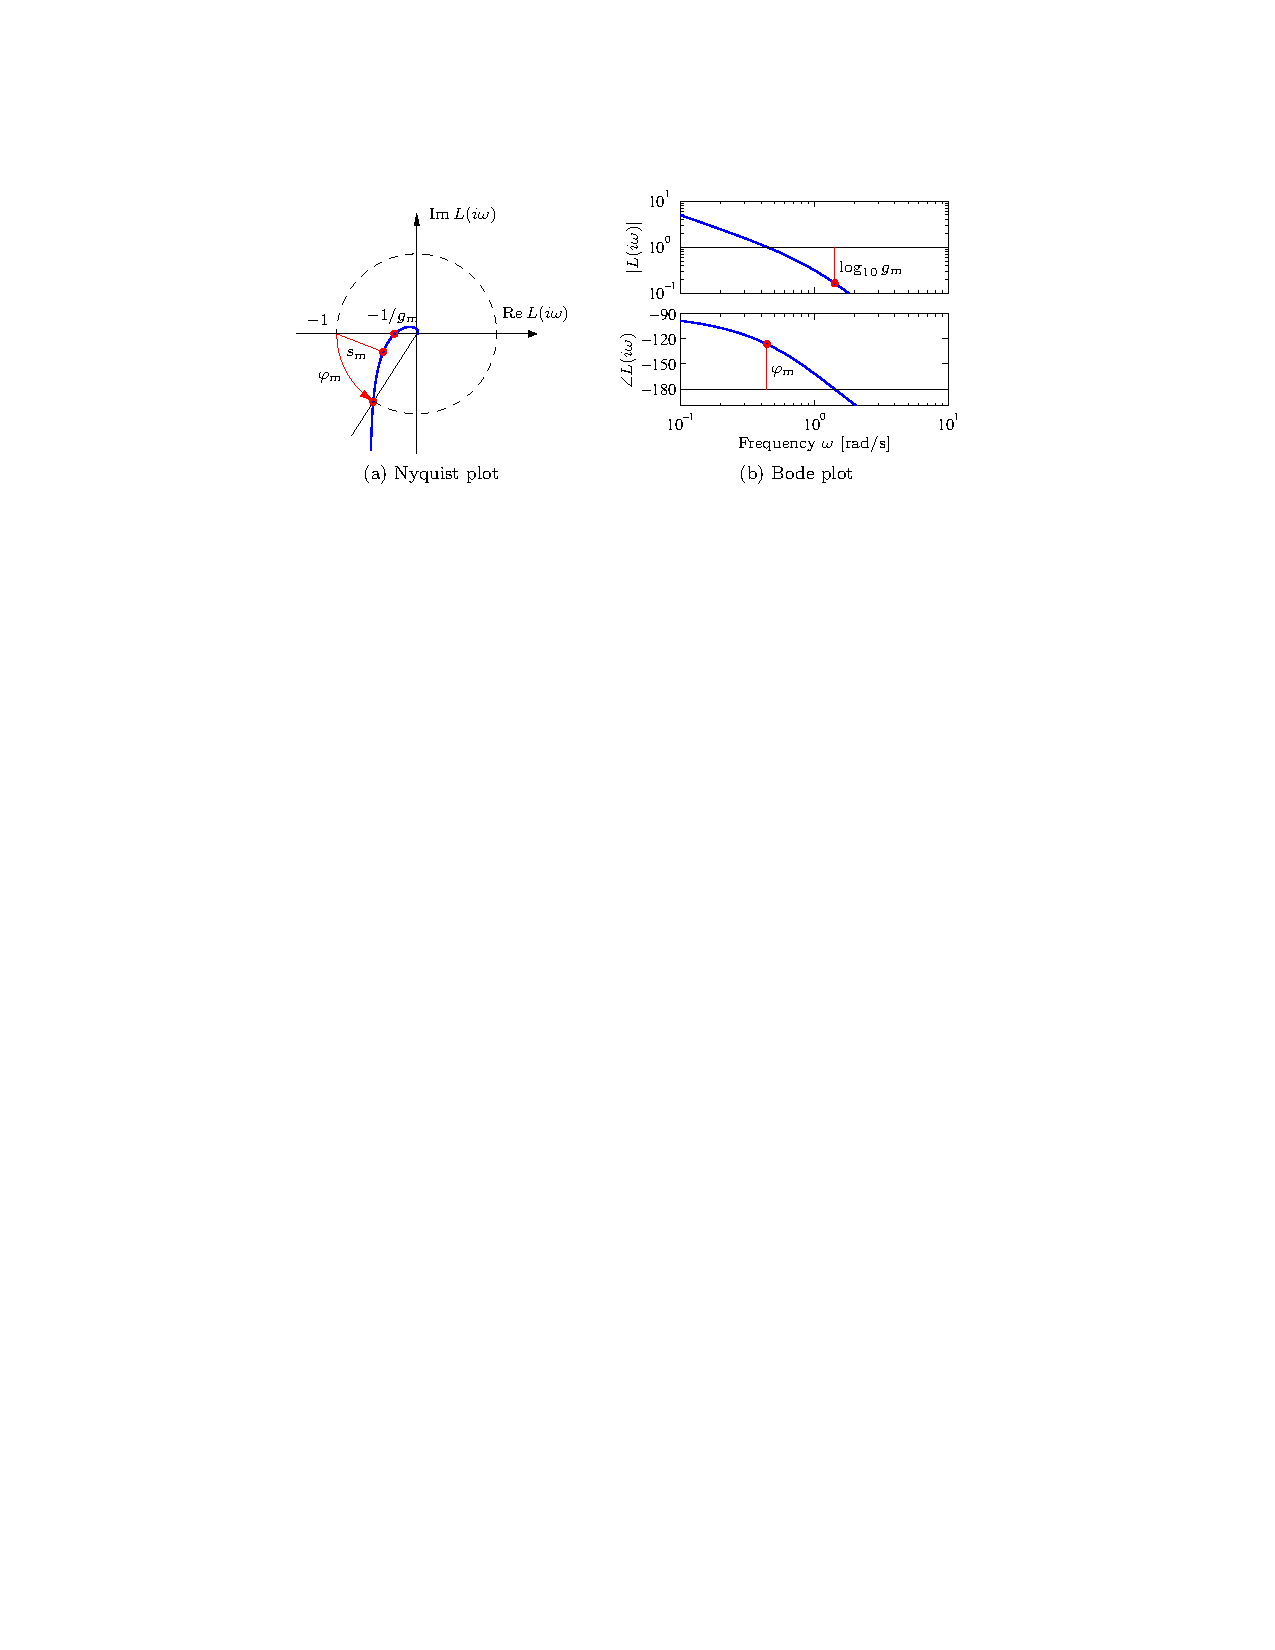
\includegraphics[width=0.9\linewidth]{figure10.11}
	\\
	\textbf{Figure 10.11:} Stability margins for a third-order loop transfer function.
\end{figure}
\end{frame}


\begin{frame}{Example}
\begin{itemize}
	\item Consider the loop transfer function $L=\tfrac{3}{(s+1)^3}$
	\item From the Nyquist plot we get $s_m=0.464$, $g_m = 2.67$, $\varphi=41.7^\circ$
\end{itemize}
\begin{figure}
	\centering
	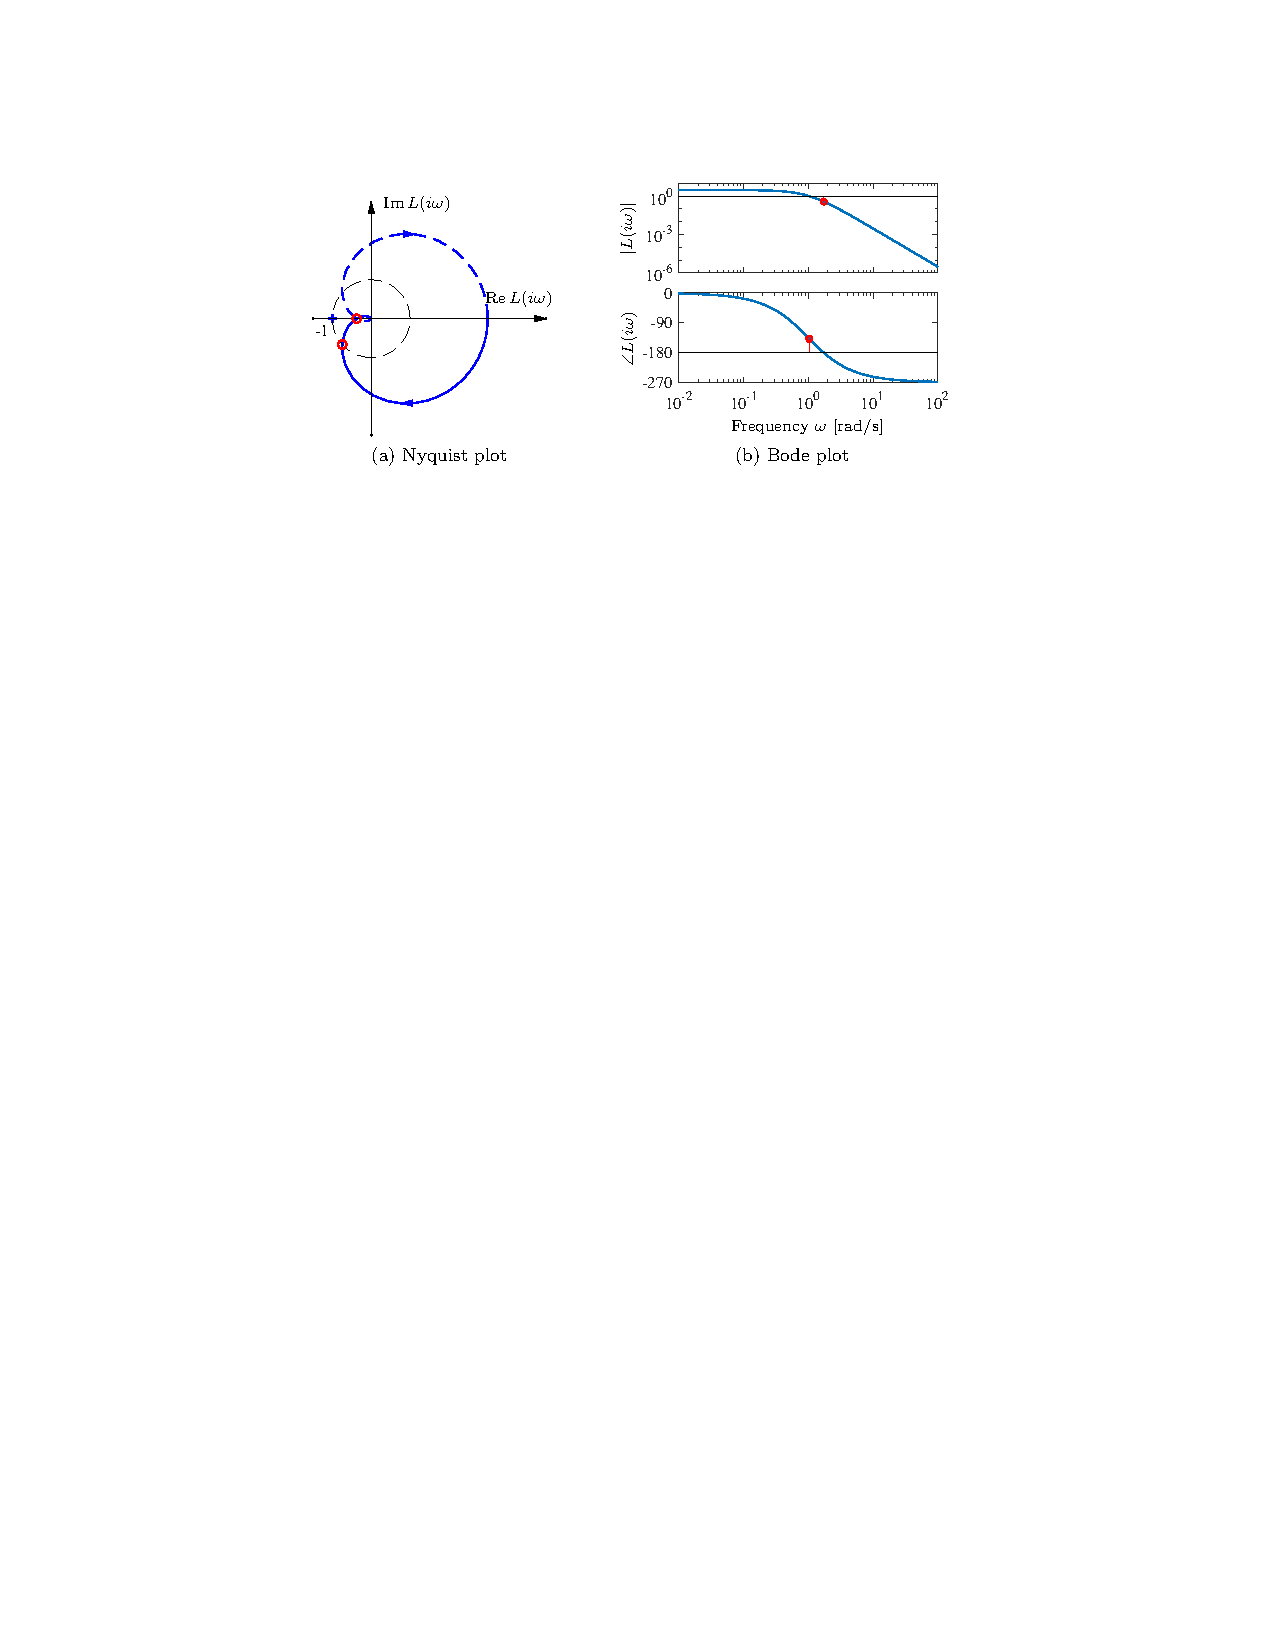
\includegraphics[width=0.9\linewidth]{figure10.12}
	\\
	\textbf{Figure 10.12:} Stability margins for a third-order loop transfer function.
\end{figure}
\end{frame}

\SUMMARYFRAME
\FINALE

\end{document}
